\documentclass[11pt,a4paper]{article}

\usepackage[margin=1in]{geometry}
\usepackage{amsmath,amssymb,amsthm}
\usepackage{booktabs}
\usepackage{pgfplots}
\pgfplotsset{compat=1.18}
\usepgfplotslibrary{groupplots}
\usepackage[round]{natbib}
\usepackage[colorlinks=true,linkcolor=black,citecolor=black,urlcolor=blue]{hyperref}
\usepackage{parskip}
\usepackage{caption}

\newtheorem{proposition}{Proposition}
\newcommand{\E}{\mathbb{E}}
\setlength{\emergencystretch}{1.5em}

\title{\textbf{From Gross Edge to Net Profit}\\[0.4em]
\large Fill Timing and Trading Costs in an Intraday Reversal Strategy}
\author{Khanh Nguyen}
\date{}

\begin{document}
\maketitle

\begin{abstract}
\noindent A 5-minute direction model on 431 S\&P~500 stocks has a steady gross edge: filled at the
close of the bar that produced the signal, \$1 million grows to \$4{,}091{,}721 in 4.05 years with a
Sharpe ratio of $9.01$ and a worst drawdown of $-2.2\%$. This paper asks how much of that survives
execution. We make three contributions. First, we prove that the difference between filling at the
signal bar's close and at the next bar's open equals position change times the jump between the two
prints, and show that this jump is bid--ask bounce: it removes $46\%$ of the gross edge. Second, we
measure trading costs per stock and per day from the bars themselves, including an exact lower bound: no
market order can pay less than half a \$0.01 tick. Third, we test whether trading less, trading
tight-spread stocks, or combining timeframes rescues the strategy. It does not. Every one of the
46 versions tested loses money at the lower-bound cost; the best out-of-sample version turns \$1
million into \$870{,}953 over 2022--2025. The edge grows with the spread, but a follow-up test shows that
limit orders resting at the last price do not collect it: their fills are adversely selected.
\end{abstract}

%=====================================================================
\section{Introduction}
\label{sec:intro}

\paragraph{Motivation.} Most strategies that look good in a backtest lose money when traded. For
high-frequency strategies the main reason is simple: they trade often, and each trade costs money.
\citet{novymarx2016} show that trading costs remove most of the profit of many published anomalies with
high turnover. Intraday strategies turn over their whole book many times a day, so a cost of a fraction
of a basis point per trade decides the result. Yet backtests often ignore costs or charge one flat
number, and often assume a fill at the very price that produced the signal.

\paragraph{Reversal and the spread.} Short-horizon returns reverse
\citep{lehmann1990}. Part of this is bid--ask bounce: a trade at the bid followed by a trade at the ask
looks like a reversal even when the value has not changed \citep{roll1984}. Bounce explains much of
short-horizon reversal \citep{kaul1990,jegadeesh1995}, and reversal profits can be read as the return to
providing liquidity \citep{nagel2012}. A reversal strategy measured on
traded prices may therefore be measuring the spread, which a liquidity taker pays rather than earns.

\paragraph{This paper.} We take a model with a real and steady gross edge, a multi-timeframe ARX on
5-minute bars described in Section~\ref{sec:strategy}, and follow its profit from the backtest to what a
trader would actually get. We ask three questions. How much of the gross edge depends on the assumed
fill price? What does the strategy cost to trade, measured per stock and per day? And can any version,
by trading less or trading only cheap stocks, pay for itself?

\paragraph{Findings.}
\begin{enumerate}
\item \textbf{About half the gross edge is the fill assumption} (Section~\ref{sec:fill}). Moving the fill
from the signal bar's close to the next bar's open, one print later, removes $46\%$ of the 5-minute
edge. We prove the difference equals position change times the jump from the close to the next open,
and show that this jump reverses the last bar's move in $94\%$ of stocks after down bars.
\item \textbf{Every version loses money at the smallest possible cost} (Section~\ref{sec:results}). Half a
\$0.01 tick is a cost no market order can avoid. At that cost all 46 versions lose money.
\item \textbf{The edge is the spread.} Gross breakeven rises from $0.066$ to $0.197$ bps from the
tightest to the widest spread quintile, and correlates $0.63$ with each stock's spread.
\item \textbf{The result is statistically solid.} Bootstrap confidence intervals for the net return lie
below zero; the gross edge survives a correction for 102 trials (deflated Sharpe $0.978$).
\end{enumerate}

%=====================================================================
\section{The strategy in brief}
\label{sec:strategy}

\paragraph{Forecast.} For each stock and each of six timeframes (5 minutes to 4 hours), a linear
regression forecasts the next bar's close-to-close return from five lags of return and five lags of a
bounded bar-level flow proxy, $\tanh(\operatorname{sign}(C-O)\cdot|C-O|/(H-L)\cdot\log(1+V))$. Each forecast
is divided by recent volatility, bounded with $\tanh$, and the six scores are averaged, with equal weights
or with weights learned on 2021 only. Models are refitted monthly on the previous year.

\paragraph{Positions.} Long one unit if the score is positive, short if negative (``sign''); or a position
equal to the score (``size''); or the sign only when the score is in the top quarter of its recent
distribution, holding the previous position otherwise (``filtered''). ``CLOSE 5m'' is the 5-minute
timeframe alone.

\paragraph{Book and period.} 431 stocks with 5-minute regular-hours bars, equal weight,
426.6 stocks per bar on average, 2020-12-18 to 2025-01-10 (4.05 years); 2022--2025 is a hold-out for
the learned weights. Positions are closed at every session end. A look-ahead test, run on truncated
data and shown to catch a deliberate leak, confirms that no decision uses later data.

\paragraph{What the signal is.} The coefficient on the latest return is negative in $76\%$ of
monthly refits; the flow coefficients are coin flips. The model is a one-bar reversal.

%=====================================================================
\section{Fill timing}
\label{sec:fill}

\subsection{Three fill rules}

A decision is made at the end of 5-minute bar $t$, with position $w_t$ held into bar $t+1$. We compare:
\begin{itemize}
\item \textbf{Close fill}: trade at $C_t$, the last price of the signal bar. Profit $w_t\,(C_t\to C_{t+1})$.
This is the usual backtest convention.
\item \textbf{Next-open fill}: trade at $O_{t+1}$, the first print after the signal, which is what a market
order sent at the bar close receives. The old position $w_{t-1}$ is held from $C_t$ to $O_{t+1}$, the new
one from $O_{t+1}$ to $C_{t+1}$.
\item \textbf{One-bar delay}: trade at $C_{t+1}$, a signal one bar stale.
\end{itemize}
Returns are in bps of log price, so $(C_t\to C_{t+1}) = (C_t\to O_{t+1}) + (O_{t+1}\to C_{t+1})$ exactly.

\begin{proposition}[What the close fill adds]
\label{prop:fill}
Per bar, profit with the close fill minus profit with the next-open fill equals
$(w_t-w_{t-1})\cdot(C_t\to O_{t+1})$.
\end{proposition}
\begin{proof}
Close fill: $w_t(C_t\to O_{t+1}) + w_t(O_{t+1}\to C_{t+1})$. Next-open fill:
$w_{t-1}(C_t\to O_{t+1}) + w_t(O_{t+1}\to C_{t+1})$. Subtract.
\end{proof}

The close fill therefore earns extra exactly when the position changes in the direction of the jump
from the close to the next print. For a reversal strategy the position changes after a bar moved: after a
down bar it buys. If the close of a down bar tends to be printed at the bid, the next print is higher,
and the close fill credits the strategy with a gain that the buyer, who pays the ask, never gets.

\paragraph{The jump is bounce.} The move from the close to the next print averages $-0.112$ bps after up
bars and $+0.148$ bps after down bars: it goes against the last bar in $87\%$ and $94\%$ of
stocks respectively. The
first print after the close moves back towards the middle of the spread, as \citet{roll1984} predicts
for prints that alternate between bid and ask.

\begin{table}[htbp]
\centering
\caption{Breakeven half-spread (bps) under each fill rule, and gross Sharpe ratio. Breakeven is gross
profit per bar divided by turnover per bar.}
\label{tab:fill}
\small
\begin{tabular}{@{}lrrrrr@{}}
\toprule
& \multicolumn{3}{c}{Breakeven (bps)} & \multicolumn{2}{c}{Gross Sharpe} \\
\cmidrule(lr){2-4}\cmidrule(lr){5-6}
Strategy & Close fill & Next open & 1-bar delay & Close fill & Next open \\
\midrule
CLOSE 5m & $0.190$ & $0.103$ & $0.030$ & $9.01$ & $4.99$ \\
CLOSE MTF, equal, sign & $0.318$ & $0.182$ & $0.086$ & $6.24$ & $3.61$ \\
CLOSE MTF, equal, filtered & $0.590$ & $0.280$ & $0.125$ & $2.76$ & $1.32$ \\
CLOSE 4h only & $0.566$ & $0.558$ & $0.577$ & $1.46$ & $1.44$ \\
MID 5m & $-0.243$ & $-0.133$ & $-0.057$ & $-7.35$ & $-4.14$ \\
\midrule \multicolumn{6}{@{}l}{\textit{Out of sample, Jan 2022 -- Jan 2025}} \\
CLOSE MTF, learned, filtered & $0.563$ & $0.219$ & $0.095$ & $2.07$ & $0.81$ \\
\bottomrule
\end{tabular}
\end{table}

\paragraph{Reading Table~\ref{tab:fill}.} For CLOSE 5m, the close fill earns $0.181$ bps per bar and the
next-open fill $0.098$; the difference, $0.083$ bps, is the term of Proposition~\ref{prop:fill}, and
is $46\%$ of the close-fill edge ($53\%$ for the filtered book). Across strategies the
breakeven falls by $43\%$--$65\%$. With a one-bar delay almost nothing is left: the signal's
information lasts about one bar. The 4-hour model is the exception: it trades rarely, so the fill hardly
matters. All results below use the next-open fill.

%=====================================================================
\section{Trading costs}
\label{sec:costs}

\subsection{Net profit and breakeven}

With half-spread $c$ (in bps) and turnover $|w_t-w_{t-1}|$, the net profit of a bar is
gross profit $-\,c\cdot|w_t-w_{t-1}|$. A switch from long to short counts two and pays two half-spreads. The
breakeven half-spread is gross profit per bar divided by turnover per bar: the largest cost at which the
book still breaks even. A high Sharpe ratio built from small bets can coexist with a very low breakeven,
so breakeven, not Sharpe, decides whether a strategy can be traded.

\subsection{Three cost measures}

We have no quote data, so costs are measured from the bars. All three measures are computed per stock
and per day from data before that day.

\paragraph{Tick floor (exact lower bound).} Prices move in \$0.01 ticks, so the quoted spread is at least
one tick and a market order pays at least half a tick: $c^{\text{tick}} = 0.005/P\times10^4$ bps, with $P$
the previous session's close. This is not an estimate. If a strategy loses money at this cost, it loses
money at every real cost.

\paragraph{Abdi--Ranaldo (central estimate).} \citet{abdi2017} note that the distance between the close
and the midpoint of the range, $c_t-\eta_t$ with $\eta=(h+l)/2$ in logs, contains half the spread with a
random sign, and that this sign is independent across bars. Hence
$S^2 = 4\,\E[(c_t-\eta_t)(c_t-\eta_{t+1})]$. We average the products over the previous
20 sessions and take the square root (zero if negative). The estimator uses the close, so it
measures exactly the kind of bounce a reversal strategy trades on.

\paragraph{Corwin--Schultz (upper estimate).} \citet{corwin2012} use the fact that the high--low range of
one bar contains the variance once and the spread once, while the range over two bars contains the
variance twice and the spread still once. Two equations give the spread. We apply it to consecutive
5-minute bars, set negative values to zero and average over the previous 20 sessions. The
estimator assumes the price moves continuously within the bar, which fails for short, thinly traded bars
and biases it upwards when volatility is high.

\begin{table}[htbp]
\centering
\caption{Half-spreads across stocks (bps), average over the sample for each stock.}
\label{tab:costdist}
\small
\begin{tabular}{@{}lrrrrr@{}}
\toprule
Measure & 10\% & 25\% & Median & 75\% & 90\% \\
\midrule
Tick floor (lower bound) & $0.15$ & $0.25$ & $0.47$ & $0.81$ & $1.36$ \\
Abdi--Ranaldo (central) & $0.98$ & $1.25$ & $1.59$ & $2.05$ & $2.85$ \\
Corwin--Schultz (upper) & $1.59$ & $1.90$ & $2.31$ & $2.83$ & $3.71$ \\
\bottomrule
\end{tabular}
\end{table}

\paragraph{Reading Table~\ref{tab:costdist}.} Liquid large caps usually quote one or a few ticks wide.
The Abdi--Ranaldo median of $1.59$ bps is a few times the tick floor, which is plausible. The
Corwin--Schultz median of $2.31$ bps is too high for stocks this liquid; its largest values are for the
most volatile names (ENPH, CCL, MRNA), consistent with its volatility bias. We therefore base the verdict on
the tick floor, use Abdi--Ranaldo as the central case, and report Corwin--Schultz only as an upper
estimate. This rule was fixed before the cost results were seen.

%=====================================================================
\section{Results}
\label{sec:results}

\subsection{The edge grows with the spread}

\begin{table}[htbp]
\centering
\caption{Stocks split each day into quintiles of their past Abdi--Ranaldo spread (q1 tightest).
Next-open fill. The split was fixed before the results were seen.}
\label{tab:bkt}
\small
\begin{tabular}{@{}lrrrrr@{}}
\toprule
& q1 & q2 & q3 & q4 & q5 \\
\midrule
\multicolumn{6}{@{}l}{\textit{Gross breakeven, next-open fill (bps)}} \\
CLOSE 5m & $0.066$ & $0.049$ & $0.086$ & $0.114$ & $0.197$ \\
MTF, equal, filtered & $0.135$ & $0.095$ & $0.126$ & $0.452$ & $0.553$ \\
MTF, learned, filtered & $0.113$ & $0.226$ & $0.241$ & $0.365$ & $0.620$ \\
\midrule \multicolumn{6}{@{}l}{\textit{Total return after the tick floor}} \\
CLOSE 5m & $-73\%$ & $-44\%$ & $-54\%$ & $-53\%$ & $-54\%$ \\
MTF, equal, filtered & $-8\%$ & $-4\%$ & $-5\%$ & $-2\%$ & $-2\%$ \\
\midrule \multicolumn{6}{@{}l}{\textit{Total return after Abdi--Ranaldo costs (the ranking variable)}} \\
CLOSE 5m & $+1\%$ & $-67\%$ & $-90\%$ & $-97\%$ & $-100\%$ \\
MTF, equal, filtered & $+1\%$ & $-7\%$ & $-15\%$ & $-19\%$ & $-31\%$ \\
\bottomrule
\end{tabular}
\end{table}

\paragraph{Reading Table~\ref{tab:bkt}.} Gross breakeven is lowest in the tightest-spread stocks and
highest in the widest: $0.066$ to $0.197$ bps for CLOSE 5m, $0.135$ to $0.553$ for the
filtered book. Across stocks, breakeven correlates $0.63$ with the stock's spread. A signal that is
strongest where the spread is widest is harvesting the spread.

\paragraph{Trading only cheap stocks does not help.} Under Abdi--Ranaldo costs the tightest quintile
roughly breaks even ($+1\%$ for CLOSE 5m). This is not credible: the same noisy estimate chooses the
stocks and sets their cost, so stocks whose spread is under-estimated are chosen and then under-charged.
At the tick floor, which has no estimation error, the same quintile returns $-73\%$.

\paragraph{Per stock.} Only $11\%$ of stocks have a 5-minute breakeven above their own tick floor
($37\%$ for the filtered book), and $0\%$ ($6\%$) above their own Abdi--Ranaldo spread.

\subsection{Performance in dollars}

\begin{center}
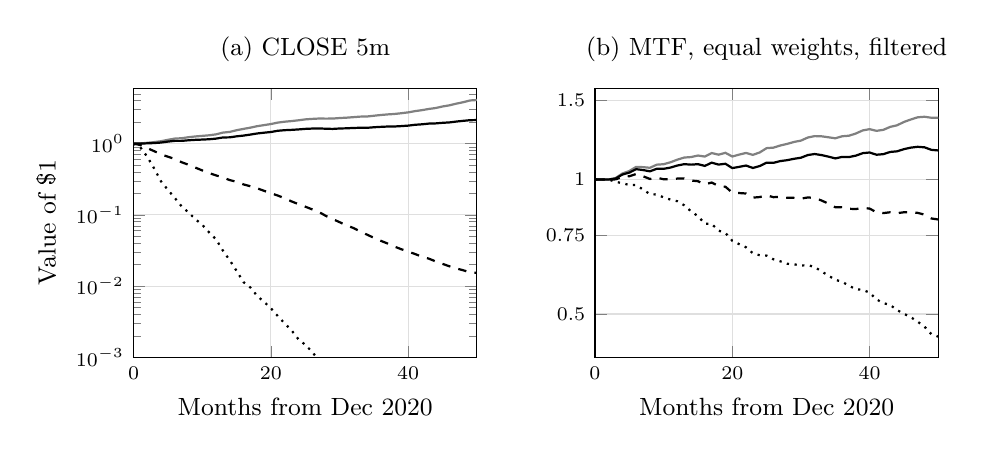
\begin{tikzpicture}
\begin{groupplot}[group style={group size=2 by 1, horizontal sep=1.5cm},
  width=0.49\textwidth, height=5cm, ymode=log, grid=major, grid style={gray!25},
  xlabel={Months from Dec 2020}, xmin=0, xmax=50,
  legend style={font=\scriptsize, legend columns=4, /tikz/every even column/.append style={column sep=6pt}},
  tick label style={font=\scriptsize}, label style={font=\small}, title style={font=\small}]
\nextgroupplot[title={(a) CLOSE 5m}, ylabel={Value of \$1}, ymin=0.001, ymax=6]
\addplot[thick, gray] coordinates {(0,1) (1,1.0067) (2,1.0268) (3,1.0511) (4,1.0813) (5,1.1309) (6,1.1766) (7,1.1908) (8,1.2300) (9,1.2610) (10,1.2845) (11,1.3090) (12,1.3490) (13,1.4276) (14,1.4602) (15,1.5418) (16,1.6092) (17,1.6751) (18,1.7573) (19,1.8186) (20,1.8829) (21,1.9736) (22,2.0310) (23,2.0715) (24,2.1244) (25,2.1883) (26,2.2238) (27,2.2498) (28,2.2433) (29,2.2473) (30,2.2860) (31,2.3125) (32,2.3516) (33,2.3935) (34,2.4032) (35,2.4625) (36,2.5212) (37,2.5705) (38,2.6076) (39,2.6716) (40,2.7457) (41,2.8599) (42,2.9496) (43,3.0661) (44,3.1603) (45,3.3224) (46,3.4490) (47,3.6394) (48,3.8106) (49,4.0341) (50,4.0917)};
\addplot[thick, black] coordinates {(0,1) (1,1.0024) (2,1.0095) (3,1.0185) (4,1.0353) (5,1.0683) (6,1.0932) (7,1.0931) (8,1.1142) (9,1.1300) (10,1.1397) (11,1.1516) (12,1.1753) (13,1.2193) (14,1.2252) (15,1.2660) (16,1.2962) (17,1.3390) (18,1.3882) (19,1.4233) (20,1.4556) (21,1.5147) (22,1.5439) (23,1.5600) (24,1.5816) (25,1.6110) (26,1.6264) (27,1.6319) (28,1.6190) (29,1.6085) (30,1.6304) (31,1.6403) (32,1.6587) (33,1.6692) (34,1.6665) (35,1.6972) (36,1.7193) (37,1.7370) (38,1.7404) (39,1.7619) (40,1.7899) (41,1.8391) (42,1.8667) (43,1.9100) (44,1.9231) (45,1.9593) (46,1.9844) (47,2.0400) (48,2.0883) (49,2.1326) (50,2.1416)};
\addplot[thick, black, dashed] coordinates {(0,1) (1,0.9557) (2,0.8635) (3,0.7840) (4,0.7066) (5,0.6557) (6,0.6086) (7,0.5480) (8,0.5048) (9,0.4606) (10,0.4206) (11,0.3855) (12,0.3583) (13,0.3352) (14,0.3077) (15,0.2912) (16,0.2678) (17,0.2522) (18,0.2358) (19,0.2177) (20,0.2007) (21,0.1868) (22,0.1711) (23,0.1546) (24,0.1417) (25,0.1304) (26,0.1195) (27,0.1096) (28,0.0968) (29,0.0874) (30,0.0790) (31,0.0713) (32,0.0655) (33,0.0587) (34,0.0528) (35,0.0476) (36,0.0433) (37,0.0396) (38,0.0359) (39,0.0329) (40,0.0305) (41,0.0282) (42,0.0259) (43,0.0243) (44,0.0222) (45,0.0205) (46,0.0190) (47,0.0177) (48,0.0167) (49,0.0156) (50,0.0153)};
\addplot[thick, black, dotted] coordinates {(0,1) (1,0.8816) (2,0.6533) (3,0.4470) (4,0.2952) (5,0.2244) (6,0.1731) (7,0.1314) (8,0.1081) (9,0.0870) (10,0.0726) (11,0.0568) (12,0.0456) (13,0.0316) (14,0.0231) (15,0.0164) (16,0.0114) (17,0.0096) (18,0.0073) (19,0.0060) (20,0.0049) (21,0.0038) (22,0.0030) (23,0.0024) (24,0.0018) (25,0.0015) (26,0.0012) (27,0.0009) (28,0.0008) (29,0.0007) (30,0.0006) (31,0.0005) (32,0.0004) (33,0.0003) (34,0.0003) (35,0.0002) (36,0.0002) (37,0.0001) (38,0.0001) (39,0.0001) (40,0.0001) (41,0.0001) (42,0.0000) (43,0.0000) (44,0.0000) (45,0.0000) (46,0.0000) (47,0.0000) (48,0.0000) (49,0.0000) (50,0.0000)};
\nextgroupplot[title={(b) MTF, equal weights, filtered}, ymin=0.4, ymax=1.6, ytick={0.5,0.75,1,1.5},
  yticklabels={0.5,0.75,1,1.5}, legend to name=eqleg]
\addplot[thick, gray] coordinates {(0,1) (1,1.0000) (2,0.9996) (3,1.0071) (4,1.0311) (5,1.0444) (6,1.0668) (7,1.0654) (8,1.0618) (9,1.0791) (10,1.0816) (11,1.0925) (12,1.1072) (13,1.1193) (14,1.1222) (15,1.1310) (16,1.1250) (17,1.1457) (18,1.1360) (19,1.1470) (20,1.1253) (21,1.1364) (22,1.1461) (23,1.1349) (24,1.1493) (25,1.1749) (26,1.1779) (27,1.1911) (28,1.2009) (29,1.2130) (30,1.2214) (31,1.2410) (32,1.2500) (33,1.2487) (34,1.2425) (35,1.2360) (36,1.2490) (37,1.2525) (38,1.2670) (39,1.2872) (40,1.2955) (41,1.2843) (42,1.2911) (43,1.3108) (44,1.3216) (45,1.3445) (46,1.3618) (47,1.3772) (48,1.3809) (49,1.3739) (50,1.3732)}; \addlegendentry{close fill, gross}
\addplot[thick, black] coordinates {(0,1) (1,1.0000) (2,0.9996) (3,1.0047) (4,1.0257) (5,1.0358) (6,1.0543) (7,1.0495) (8,1.0427) (9,1.0565) (10,1.0562) (11,1.0631) (12,1.0744) (13,1.0819) (14,1.0792) (15,1.0818) (16,1.0722) (17,1.0903) (18,1.0795) (19,1.0841) (20,1.0602) (21,1.0670) (22,1.0742) (23,1.0608) (24,1.0716) (25,1.0904) (26,1.0894) (27,1.0992) (28,1.1043) (29,1.1122) (30,1.1184) (31,1.1339) (32,1.1399) (33,1.1336) (34,1.1247) (35,1.1144) (36,1.1230) (37,1.1223) (38,1.1304) (39,1.1449) (40,1.1489) (41,1.1357) (42,1.1391) (43,1.1521) (44,1.1558) (45,1.1688) (46,1.1780) (47,1.1830) (48,1.1798) (49,1.1646) (50,1.1610)}; \addlegendentry{next-open fill, gross}
\addplot[thick, black, dashed] coordinates {(0,1) (1,1.0000) (2,0.9995) (3,1.0003) (4,1.0135) (5,1.0166) (6,1.0285) (7,1.0165) (8,1.0024) (9,1.0087) (10,1.0010) (11,1.0009) (12,1.0044) (13,1.0045) (14,0.9944) (15,0.9909) (16,0.9750) (17,0.9841) (18,0.9666) (19,0.9631) (20,0.9341) (21,0.9323) (22,0.9301) (23,0.9106) (24,0.9133) (25,0.9214) (26,0.9127) (27,0.9146) (28,0.9100) (29,0.9095) (30,0.9058) (31,0.9114) (32,0.9092) (33,0.8971) (34,0.8829) (35,0.8667) (36,0.8671) (37,0.8597) (38,0.8587) (39,0.8635) (40,0.8607) (41,0.8442) (42,0.8409) (43,0.8445) (44,0.8405) (45,0.8445) (46,0.8449) (47,0.8418) (48,0.8342) (49,0.8179) (50,0.8136)}; \addlegendentry{next open, tick floor}
\addplot[thick, black, dotted] coordinates {(0,1) (1,1.0000) (2,0.9993) (3,0.9878) (4,0.9808) (5,0.9716) (6,0.9717) (7,0.9490) (8,0.9274) (9,0.9252) (10,0.9118) (11,0.9014) (12,0.8938) (13,0.8753) (14,0.8484) (15,0.8276) (16,0.7963) (17,0.7952) (18,0.7684) (19,0.7593) (20,0.7292) (21,0.7168) (22,0.7051) (23,0.6836) (24,0.6767) (25,0.6755) (26,0.6627) (27,0.6560) (28,0.6477) (29,0.6459) (30,0.6419) (31,0.6431) (32,0.6372) (33,0.6227) (34,0.6095) (35,0.5964) (36,0.5904) (37,0.5784) (38,0.5682) (39,0.5663) (40,0.5583) (41,0.5391) (42,0.5290) (43,0.5239) (44,0.5102) (45,0.5007) (46,0.4919) (47,0.4807) (48,0.4684) (49,0.4506) (50,0.4451)}; \addlegendentry{next open, Abdi--Ranaldo}
\end{groupplot}
\end{tikzpicture}\\[-2pt]
\ref{eqleg}
\captionof{figure}{Growth of \$1, log scale, month-end values. Grey to solid: the fill assumption. Solid
to dashed: the smallest possible cost. Dashed to dotted: a realistic cost.}
\label{fig:eq}
\end{center}

\begin{table}[htbp]
\centering
\caption{\$1{,}000{,}000 at the start, compounded bar by bar, 2020-12-18 to 2025-01-10. ``Vol'' is annual
volatility; ``Max DD'' the largest fall from a peak; last column: share of months with a gain.}
\label{tab:perf}
\footnotesize
\setlength{\tabcolsep}{3pt}
\begin{tabular}{@{}llrrrrrrr@{}}
\toprule
Strategy & Fill, cost & End value & Total & CAGR & Vol & Sharpe & Max DD & Mo.\ $>0$ \\
\midrule
CLOSE 5m & close fill, gross & \$4{,}091{,}721 & $+309.2\%$ & $+41.6\%$ & $3.9\%$ & $9.01$ & $-2.2\%$ & $98\%$ \\
 & next open, gross & \$2{,}141{,}607 & $+114.2\%$ & $+20.7\%$ & $3.8\%$ & $4.99$ & $-2.6\%$ & $92\%$ \\
 & next open, tick floor & \$15{,}298 & $-98.5\%$ & $-64.4\%$ & $3.9\%$ & $-27.25$ & $-98.5\%$ & $0\%$ \\
 & next open, AR & \$4 & $-100.0\%$ & $-95.3\%$ & $3.9\%$ & $-79.05$ & $-100.0\%$ & $0\%$ \\
 & next open, 0.87 bps & \$3{,}305 & $-99.7\%$ & $-75.6\%$ & $3.9\%$ & $-37.25$ & $-99.7\%$ & $0\%$ \\
\midrule
MTF, equal, sign & close fill, gross & \$2{,}157{,}954 & $+115.8\%$ & $+20.9\%$ & $3.1\%$ & $6.24$ & $-2.0\%$ & $96\%$ \\
 & next open, gross & \$1{,}552{,}316 & $+55.2\%$ & $+11.5\%$ & $3.1\%$ & $3.61$ & $-2.3\%$ & $84\%$ \\
 & next open, tick floor & \$309{,}890 & $-69.0\%$ & $-25.1\%$ & $3.1\%$ & $-9.53$ & $-69.3\%$ & $0\%$ \\
 & next open, AR & \$19{,}949 & $-98.0\%$ & $-62.0\%$ & $3.2\%$ & $-30.98$ & $-98.0\%$ & $0\%$ \\
 & next open, 0.87 bps & \$188{,}775 & $-81.1\%$ & $-33.8\%$ & $3.1\%$ & $-13.53$ & $-81.3\%$ & $0\%$ \\
\midrule
MTF, equal, filtered & close fill, gross & \$1{,}373{,}183 & $+37.3\%$ & $+8.2\%$ & $2.9\%$ & $2.76$ & $-2.9\%$ & $72\%$ \\
 & next open, gross & \$1{,}160{,}997 & $+16.1\%$ & $+3.8\%$ & $2.9\%$ & $1.32$ & $-4.1\%$ & $62\%$ \\
 & next open, tick floor & \$813{,}564 & $-18.6\%$ & $-5.0\%$ & $2.9\%$ & $-1.78$ & $-21.2\%$ & $34\%$ \\
 & next open, AR & \$445{,}066 & $-55.5\%$ & $-18.1\%$ & $2.9\%$ & $-6.89$ & $-55.6\%$ & $4\%$ \\
 & next open, 0.87 bps & \$725{,}769 & $-27.4\%$ & $-7.6\%$ & $2.9\%$ & $-2.76$ & $-29.3\%$ & $28\%$ \\
\midrule
MID 5m & close fill, gross & \$137{,}618 & $-86.2\%$ & $-38.7\%$ & $6.7\%$ & $-7.35$ & $-86.3\%$ & $10\%$ \\
 & next open, gross & \$336{,}381 & $-66.4\%$ & $-23.6\%$ & $6.6\%$ & $-4.14$ & $-66.6\%$ & $12\%$ \\
 & next open, tick floor & \$1{,}527 & $-99.8\%$ & $-79.9\%$ & $6.6\%$ & $-24.77$ & $-99.8\%$ & $0\%$ \\
 & next open, AR & \$0 & $-100.0\%$ & $-97.8\%$ & $6.6\%$ & $-58.64$ & $-100.0\%$ & $0\%$ \\
 & next open, 0.87 bps & \$287 & $-100.0\%$ & $-86.7\%$ & $6.6\%$ & $-31.15$ & $-100.0\%$ & $0\%$ \\
\bottomrule
\end{tabular}
\end{table}

\begin{table}[htbp]
\centering
\caption{Out of sample, January 2022 -- January 2025 (3.01 years): MTF, learned weights, filtered.}
\label{tab:perfoos}
\footnotesize
\setlength{\tabcolsep}{3pt}
\begin{tabular}{@{}lrrrrrrr@{}}
\toprule
Fill, cost & End value & Total & CAGR & Vol & Sharpe & Max DD & Mo.\ $>0$ \\
\midrule
close fill, gross & \$1{,}191{,}641 & $+19.2\%$ & $+6.0\%$ & $2.9\%$ & $2.07$ & $-3.0\%$ & $70\%$ \\
next open, gross & \$1{,}069{,}992 & $+7.0\%$ & $+2.3\%$ & $2.9\%$ & $0.81$ & $-3.8\%$ & $68\%$ \\
next open, tick floor & \$870{,}953 & $-12.9\%$ & $-4.5\%$ & $2.9\%$ & $-1.61$ & $-14.6\%$ & $38\%$ \\
next open, AR & \$616{,}553 & $-38.3\%$ & $-14.8\%$ & $2.9\%$ & $-5.55$ & $-38.4\%$ & $11\%$ \\
next open, 0.87 bps & \$814{,}363 & $-18.6\%$ & $-6.6\%$ & $2.9\%$ & $-2.39$ & $-19.6\%$ & $30\%$ \\
\bottomrule
\end{tabular}
\end{table}

\paragraph{CLOSE 5m.} Before costs the book is excellent: \$4{,}091{,}721 with the close fill, \$2{,}141{,}607
with the next-open fill, and volatility of only $3.8\%$ because it is long about half the stocks and short
the rest, so market moves cancel. It changes $0.95$ units of position per bar. At the median tick floor
that alone costs about $0.450$ bps per bar, close to its whole gross return, and the book ends at
\$15{,}298. A high Sharpe ratio and a near-total loss are both correct: many tiny bets, each costing
more to place than it earns.

\paragraph{MTF, filtered.} Trading far less, it keeps more: \$1{,}160{,}997 gross, \$813{,}564 after the tick
floor ($-19\%$, worst drawdown $-21.2\%$), \$445{,}066 after Abdi--Ranaldo costs. Out of sample
with learned weights (Table~\ref{tab:perfoos}) it ends at \$1{,}069{,}992 before costs and \$870{,}953
after the tick floor.

\paragraph{MID 5m} uses the midpoint of the range as its price and loses money before any cost
(\$336{,}381 with the next-open fill). Its apparent accuracy comes from a known term in the midpoint
return, not from information.

\subsection{Statistical confidence}

\begin{table}[htbp]
\centering
\caption{95\% confidence intervals, moving-block bootstrap over trading days \citep{kunsch1989}
(20-day blocks, 1{,}000 draws), next-open fill.}
\label{tab:ci}
\footnotesize
\setlength{\tabcolsep}{3pt}
\begin{tabular}{@{}lrrrr@{}}
\toprule
& & & \multicolumn{2}{c}{After the tick floor (\%)} \\
\cmidrule(lr){4-5}
Strategy & Gross Sharpe & Breakeven (bps) & CAGR & Max DD \\
\midrule
CLOSE 5m & $[4.10,\ 5.97]$ & $[0.083,\ 0.122]$ & $[-66.0,\ -62.8]$ & $[-98.7,\ -98.2]$ \\
MTF, equal, sign & $[2.66,\ 4.66]$ & $[0.134,\ 0.233]$ & $[-27.5,\ -22.8]$ & $[-72.8,\ -65.0]$ \\
MTF, equal, filtered & $[0.32,\ 2.39]$ & $[0.068,\ 0.504]$ & $[-7.7,\ -2.1]$ & $[-28.7,\ -10.8]$ \\
CLOSE 4h only & $[0.19,\ 2.87]$ & $[0.075,\ 1.061]$ & $[-2.9,\ 2.0]$ & $[-12.9,\ -2.4]$ \\
MTF, learned, filtered, 2022+ & $[-0.40,\ 1.97]$ & $[-0.108,\ 0.515]$ & $[-7.7,\ -1.5]$ & $[-22.2,\ -7.3]$ \\
\bottomrule
\end{tabular}
\end{table}

\paragraph{The loss is not noise.} Days are resampled in blocks to keep intraday and short-run dependence.
After the tick floor the CAGR interval lies below zero for every book except the 4-hour model alone, which
cannot be told apart from breakeven. The filtered book's breakeven interval is wide ($0.037$ to $0.516$
bps across block lengths of 5, 20 and 60 days), so small differences between combined versions are not
significant.

\paragraph{The gross edge is not an artefact of search.} Trying many versions inflates the best Sharpe
ratio \citep{harvey2016}. The deflated Sharpe ratio of \citet{bailey2014} corrects for the number of
trials and for non-normal returns. Counting every configuration run on these data, 102 including
an earlier specification search and the robustness checks, the best gross Sharpe ($6.26$) has a
deflated Sharpe probability of $0.978$. And selection cannot explain a loss: $100\%$ of the
46 configurations lose money at the tick floor.

\subsection{Risk and data quality}

\begin{table}[htbp]
\centering
\caption{Risk before costs, next-open fill. Net exposure is the average position across stocks ($+1$ long,
$-1$ short); beta and correlation are against the equal-weight return of all stocks, daily; DD days is
the longest time below a previous peak.}
\label{tab:risk}
\footnotesize
\setlength{\tabcolsep}{3pt}
\begin{tabular}{@{}lrrrrrrr@{}}
\toprule
Strategy & Net exp. & 99th pct $|$net$|$ & Gross exp. & Beta & Corr. & Max DD & DD days \\
\midrule
CLOSE 5m & $0.009$ & $0.61$ & $1.00$ & $-0.001$ & $-0.004$ & $-2.6\%$ & $83$ \\
MTF, equal, sign & $0.014$ & $0.49$ & $1.00$ & $-0.010$ & $-0.039$ & $-2.3\%$ & $60$ \\
MTF, equal, size & $0.001$ & $0.03$ & $0.04$ & $-0.000$ & $-0.008$ & $-0.2\%$ & $79$ \\
MTF, equal, filtered & $0.030$ & $0.45$ & $0.97$ & $-0.006$ & $-0.024$ & $-4.1\%$ & $191$ \\
MTF, learned, filtered & $0.011$ & $0.45$ & $0.97$ & $-0.004$ & $-0.018$ & $-3.8\%$ & $267$ \\
CLOSE 4h only & $-0.010$ & $0.55$ & $0.39$ & $0.002$ & $0.014$ & $-3.9\%$ & $367$ \\
MID 5m & $0.006$ & $0.94$ & $1.00$ & $-0.014$ & $-0.024$ & $-66.6\%$ & $1018$ \\
\bottomrule
\end{tabular}
\end{table}

\paragraph{Risk (Table~\ref{tab:risk}).} The books have no market exposure to speak of: net exposure is
close to zero on average and daily beta is near zero. Losses after costs therefore come from trading, not
from the market.

\begin{table}[htbp]
\centering
\caption{Without the 44 stocks with more than 5\% of bars where $H=L$ or more than 1\% with zero volume.
Breakeven in bps; total return after the tick floor, next-open fill.}
\label{tab:robust}
\footnotesize
\setlength{\tabcolsep}{3pt}
\begin{tabular}{@{}lrrrrrr@{}}
\toprule
& \multicolumn{2}{c}{B/E close fill} & \multicolumn{2}{c}{B/E next open} & \multicolumn{2}{c}{Total, tick floor} \\
\cmidrule(lr){2-3}\cmidrule(lr){4-5}\cmidrule(lr){6-7}
Strategy & All & Excl. & All & Excl. & All & Excl. \\
\midrule
CLOSE 5m & $0.190$ & $0.145$ & $0.103$ & $0.088$ & $-98\%$ & $-99\%$ \\
MTF, equal, sign & $0.318$ & $0.240$ & $0.182$ & $0.162$ & $-69\%$ & $-74\%$ \\
MTF, equal, filtered & $0.590$ & $0.377$ & $0.280$ & $0.222$ & $-19\%$ & $-23\%$ \\
MTF, learned, filtered & $0.649$ & $0.368$ & $0.309$ & $0.207$ & $-13\%$ & $-18\%$ \\
CLOSE 4h only & $0.566$ & $0.522$ & $0.558$ & $0.515$ & $-2\%$ & $-4\%$ \\
MID 5m & $-0.243$ & $-0.206$ & $-0.133$ & $-0.123$ & $-100\%$ & $-100\%$ \\
\bottomrule
\end{tabular}
\end{table}

\paragraph{Stale prints (Table~\ref{tab:robust}).} 44 thinly traded, high-priced stocks (e.g.\
AIZ, AVY, AZO, BKNG, CMG, CRL) have many bars in which the price does not move. Unchanged prices followed by a move look
like reversals. Without these stocks the gross edge is smaller, especially with the close fill, and every
conclusion holds. Interactive Brokers builds bars from filtered trades, so $C_t$ may not be the last print
on the consolidated tape; tick data would sharpen the fill-timing result.

\paragraph{Exploratory, not a strategy.} Looking by time of day after the results were known, the filtered
book's breakeven is highest late in the afternoon ($1.59$ bps in 15:00--15:30). This was not a
planned test and should be checked on new data before it is believed.

%=====================================================================
\section{What would make it tradable}
\label{sec:tradable}

The gross edge is real, but it is the spread. A trader who crosses the spread pays it; a trader who posts
limit orders at the bid after a down bar and at the ask after an up bar would earn it. That is a different
business. A resting order fills only when the market trades through it, and the orders that fill are
disproportionately the ones the market was about to move against (adverse selection); fills are
uncertain, queue position matters, and exchange rebates and fees change the numbers. None of this can be
measured without quote and order-book data, so we do not claim that a passive version would be
profitable. What the analysis does show is the size of the target: the book can afford to pay
at most $0.280$ bps per unit of position change, including adverse selection, to break even, while a market
order pays at least $0.47$ bps at the median stock.

\paragraph{A follow-up test on the same bars.} After this analysis we ran the simplest passive version,
under a specification fixed before the run and kept in the repository (\texttt{docs/spec}).
Each order rests at the signal bar's close and fills, at that price, only if the next bar trades strictly
through it; unfilled orders are cancelled. For the filtered book in 2022--2025, $83\%$ of orders fill,
the price moves $-4.6$ bps against an order over the bar in which it fills and $+25.3$ bps in its
favour over the bar in which it does not, and the net Sharpe ratio falls to $-15.1$, against $-2.3$
with market orders at the tick floor. Breaking even would need a rebate of $3.47$ bps per unit
traded. On these bars, resting at the last price does not collect the spread; whether better queue
position or faster cancellation would is a question for order-book data.

%=====================================================================
\section{Limitations}
\label{sec:limits}

\paragraph{Costs from bars, not quotes.} The tick floor is exact but is a lower bound; Abdi--Ranaldo and
Corwin--Schultz are estimates with known biases. Quote data would replace them.

\paragraph{No market impact.} Only the spread is charged. An equal-weight book in 431 stocks
trading every five minutes would move prices at any meaningful size, so the true cost is higher. This
makes the negative verdict conservative.

\paragraph{Selection.} The sample contains stocks with data through 2025. The set of versions was chosen
after earlier results on the same data; the deflated Sharpe ratio corrects the gross result for this but a
fresh set of stocks would be cleaner.

%=====================================================================
\section{Conclusion}

A 5-minute reversal signal with a Sharpe ratio of $9.01$ in a standard backtest loses money for any
trader who uses market orders. About half of its edge is the assumption of a fill at the signal bar's own
close, which Proposition~\ref{prop:fill} shows is exactly the bounce of the next print. The rest is smaller
than the smallest possible cost of a trade. The edge grows with the spread, combining timeframes and
filtering improve the edge per trade $1.8$ to $2.7$ times but not enough, and trading only cheap stocks
does not help once costs are measured without estimation error. The practical lessons are to fill at the
first print after the signal, to charge costs per stock with an exact lower bound, and to judge a
high-turnover strategy by its breakeven cost, not its Sharpe ratio.

\begin{thebibliography}{99}
\bibitem[Abdi and Ranaldo(2017)]{abdi2017} Abdi, F. and Ranaldo, A. (2017). A simple estimation of bid-ask spreads from daily close, high, and low prices. \emph{Review of Financial Studies}, 30(12), 4437--4480.
\bibitem[Bailey and L\'opez de Prado(2014)]{bailey2014} Bailey, D.~H. and L\'opez de Prado, M. (2014). The deflated Sharpe ratio: correcting for selection bias, backtest overfitting, and non-normality. \emph{Journal of Portfolio Management}, 40(5), 94--107.
\bibitem[Corwin and Schultz(2012)]{corwin2012} Corwin, S.~A. and Schultz, P. (2012). A simple way to estimate bid-ask spreads from daily high and low prices. \emph{Journal of Finance}, 67(2), 719--760.
\bibitem[Harvey et al.(2016)]{harvey2016} Harvey, C.~R., Liu, Y. and Zhu, H. (2016). \ldots and the cross-section of expected returns. \emph{Review of Financial Studies}, 29(1), 5--68.
\bibitem[Jegadeesh and Titman(1995)]{jegadeesh1995} Jegadeesh, N. and Titman, S. (1995). Short-horizon return reversals and the bid-ask spread. \emph{Journal of Financial Intermediation}, 4(2), 116--132.
\bibitem[Kaul and Nimalendran(1990)]{kaul1990} Kaul, G. and Nimalendran, M. (1990). Price reversals: bid-ask errors or market overreaction? \emph{Journal of Financial Economics}, 28(1--2), 67--93.
\bibitem[K\"unsch(1989)]{kunsch1989} K\"unsch, H.~R. (1989). The jackknife and the bootstrap for general stationary observations. \emph{Annals of Statistics}, 17(3), 1217--1241.
\bibitem[Lehmann(1990)]{lehmann1990} Lehmann, B.~N. (1990). Fads, martingales, and market efficiency. \emph{Quarterly Journal of Economics}, 105(1), 1--28.
\bibitem[Nagel(2012)]{nagel2012} Nagel, S. (2012). Evaporating liquidity. \emph{Review of Financial Studies}, 25(7), 2005--2039.
\bibitem[Novy-Marx and Velikov(2016)]{novymarx2016} Novy-Marx, R. and Velikov, M. (2016). A taxonomy of anomalies and their trading costs. \emph{Review of Financial Studies}, 29(1), 104--147.
\bibitem[Roll(1984)]{roll1984} Roll, R. (1984). A simple implicit measure of the effective bid-ask spread in an efficient market. \emph{Journal of Finance}, 39(4), 1127--1139.
\end{thebibliography}

\end{document}
